% %%% fs-state-model - Model

\label {fs-model-section}

In this section, we outline the lightweight deterministic model called {\em drifting state}. While it is described in details in~\cite{we2018adbis}, in this paper we mention properties, which play important roles in consistency enforcement techniques.

Determinism can be achieved in a stream processing system with the following straightforward approach:
\begin{enumerate}
    \item Preserve predefined total order of elements before each order-sensitive operation in a data flow
    \item Preserve the same order of output items
    \item Require all operations to be pure
\end{enumerate}

The order on elements can be defined using a natural order of input elements arrival, e.g., $x\in Cl(D)(a_t) < y\in Cl(D)(a_{t+1})$. If multiple elements are generated from one, the order between them is based on the order of generation. In this case, reorderings may occur only in a physical graph due to asynchronous distributed execution.

At first glance, total order maintenance is over-restrictive. It can be achieved, e.g., using buffering before each order-sensitive operation until punctuation or low watermark arrives ~\cite{Li:2008:OPN:1453856.1453890}. However, buffering can dramatically increase latency.

An underlying idea of drifting state model is a reduced set of available operations which are pure and can enforce order optimistically but are sufficient to implement any stateful streaming data flow. 
\subsection{Basic operations}

Any logical graph in the drifting state model is constructed using the following two operations:

{\bf Map} applies a user-defined function to an input item. It returns a sequence of new data items generated from the input one. An output sequence can be empty.

{\bf Grouping} stores input items into distinct buckets by the value of the input balancing function. When the next item arrives at the grouping, it is appended to the corresponding bucket. Each time the grouping outputs window-sized {\it tuple item}, which consists of the most recent (in terms of the defined order) items of this bucket. If the size of the bucket is less than the window, all items of the bucket are taken.

The following example illustrates the semantics of the operation. The grouping accepts items represented as natural numbers: 1,2,3, etc. The hash function returns 1 if the number is even and 0 otherwise. If the window is set to 3, the output elements are:

\[(1), (2), (1|3), (2|4), (1|3|5), (2|4|6), (3|5|7), (4|6|8)...\]

\subsubsection{Completeness}

Any stateful transformation can be expressed by decomposing into map and grouping operations with a cycle. Let us illustrate it by the example of sum operation. In a typical setting, each element is combined with previous state value and released. Then, the state is updated. In our model, firstly each element is grouped with previous state element into the pair. After that, map operation delivers a combined result, updates the state, and returns it to the grouping through the cycle. A comparison between the classical state handling approach and the drifting state model is shown in Figure~\ref{classical-drifting}.

\begin{figure}[htbp]
  \centering
  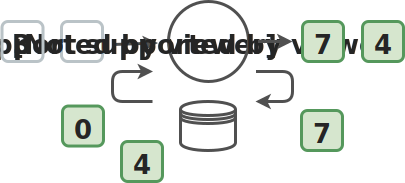
\includegraphics[width=.49\textwidth]{pics/classical-drifting}
  \caption{The comparison between typical state handling approach and drifting state model}
  \label {classical-drifting}
\end{figure}

We call this model a drifting state because operation states become ordinary data flow elements. Unlike a common approach, in this model user does not have direct access to state, and state management is done completely on the system side. Let $B$ denote a business logic operation, $x, Y$ be input and output items, $h$, the state handler and $s_t$, the state of operation $B$ at time $t$. The change in contract is illustrated in (\ref{flink-contract}).

\begin{equation}
  \label{flink-contract}
  B(x, h) = Y \qquad\Longrightarrow\qquad B(x, s_{t}) = (Y, s_{t+1}) 
\end{equation}

\subsubsection{Properties}

In this setting, map operation is pure and order insensitive, and grouping operation is pure. Grouping operation is order-sensitive because it should group a new element with the exact previous state. Hence, a straightforward approach to achieve determinism is to enforce order before grouping. Fortunately, grouping can be implemented optimistically. The scheme is shown in Figure~\ref{optimistic-grouping}. The numbers on this figure represent the right order of elements. An arriving element 3 is out-of-order. We know that actually invalid pair (1; 5) has been already released. In this case, the system generates valid pairs because the right position of the element 3 is determined. Besides, an invalid pair with a special flag is resent. Let us call such elements {\em sentinels}. While sentinels mostly behave as ordinary data items, their purpose is to seek and destroy previously released invalid pairs. Sentinels remove them from other groupings or intercept before delivery to end-user. Map functions are required to be pure in order to ensure that sentinels will go through exactly the same path as original pairs. An important property of invalid elements and corresponding sentinels is that they depend on the same input elements. This method is applicable to any number of subsequent groupings.
 
\begin{figure}[htbp]
  \centering
  \includegraphics[width=.35\textwidth]{pics/grouping-invalidation}
  \caption{An idea of optimistic grouping implementation}
  \label {optimistic-grouping}
\end{figure} 

\subsection{Output consistency}

Invalid grouping items must be destroyed by sentinels to prevent inconsistent output. Hence, the system must hold invalid elements until all corresponding sentinels arrive. In drifting state model all output items are buffered in the very last nodes of the physical graph called {\em barriers}. The problem here is to detect that there are no in-flight sentinels for elements in the barrier and they will not be generated. Invalid items and corresponding sentinels always depend on the same input element. Hence, if a system knows that all elements that depend on an input item are in the barrier, these elements can be delivered to end-user. On the other hand, as it was demonstrated in section~\ref{fs-formalism}, atomic delivery of all dependent elements is a requirement for exactly once. Therefore, the atomic releasing of dependent elements allows us to solve both problems. 

Figure~\ref{???} illustrates the concern. Elements $b^{1},b^{2},b^{3},b^{4}$ can be delivered to end-user only after the element $b^{4}$ has been processed because only in this case they can be released atomically. Otherwise, invalid grouping elements may be delivered to end-user. Another possible issue is that some elements can be applied to a system state and delivered twice in case of failure. 

\subsubsection{Dependency tracking}

Barriers require mechanisms for detecting dependencies between data flow elements. The well-known solution for dependency tracking is to inject special elements in a data flow. These elements go through the same path in a physical graph and "push through" preceding data flow elements. When such element arrives at the barrier, it means that buffered elements do not have in-flight dependencies. Flink checkpointing technique is based on this approach~\cite{Carbone:2017:SMA:3137765.3137777}. While it works well in systems that support only acyclic execution graphs, it is unclear how to handle such "pushing" elements in drifting state cycles. 

To solve this problem, each data item maintains a so-called {\em global time}. Global time is the minimal time of arrival among all input elements which affect a given one,  $GT(x)=min\{t:a_t\in Cl^{-1}(D)(x)\}$. The exact algorithms for computing and maintaining global time are detailed in~\cite{we2018adbis}, but the important property is that dependent in-flight elements have the same global time. 

On each input item, any operation in a physical graph sends to the special agent called Acker global time together with a checksum hash of the corresponding output item. Then, it sends global time and a checksum hash of the input item. Acker XORs all checksums grouped by global times and when the result becomes zero, it means that all items with a given global time were processed. In other words, it means that all derivatives of an input element with the arrival time $GT$ are in the barrier. When such event occurs, acker broadcasts a notification to the subscribers, e.g. barriers. In this approach, collisions are possible, but they are very unlikely in practice. The idea of Acker is adopted from Apache Storm~\cite{apache:storm}.

Figure~\ref{acker} illustrates acker functionality. Different shapes mean different data items. Green element is an input item. During processing, it is transformed into a blue item, and then the blue item is transformed into a yellow item. Yellow and blue items depend on the green item, so they all have the same global time (21). Each operation sends an ack for transformed items before ack for the input one to prevent XORed value become zero until all dependencies are in the barrier. For example, entry for global time 17 is zero, so it means that all dependencies of input element $a_{17}$ can be consistently released from the barrier, but for an input item $a_{21}$ there are still in-flight elements which depend on it.

\begin{figure}[htbp]
  \centering
  \includegraphics[scale=0.58]{pics/acker}
  \caption{The example of tracking dependencies using acker}
  \label {acker}
\end{figure}